\chapter{Artificial Neural Networks} 
\label{chapter-artificial} 

As we have established in the introduction, the key basis of comparison between artificial and biological neural networks is the continuity of the neural manifold. Qualitatively, we can make this comparison by visualizing both the tensor factors and the neural manifolds. Quantitatively, we can compare the mean flow ratio which provides a measure for how continuous the neural manifolds are. This chapter outlines our algorithms, key experiments, and findings for candidate models proposed in \ref{intro-framework}, which allow for a rigorous comparative analysis - these constitute our main contribution to the research literature. 

\section{CNN}
Our first candidate model is VGG16, one of the most successful CNN models in computer vision tasks such as image classification. Its architecture is shown in the figure below.
\begin{figure}[H]
    \centering
        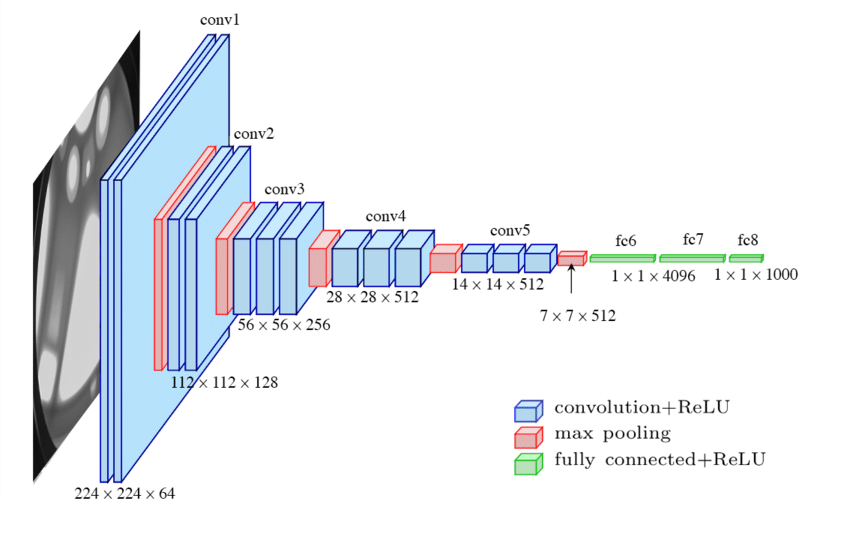
\includegraphics[width=0.5\textwidth]{figures/artificial/vgg16.png}
        \caption{Visualizing the structure of the VGG16 model.}
\end{figure}
    
\subsection{``Visual stimuli" in CNN}
Analogous to the flow stimuli in lab experiments, the ``visual stimuli" for CNN are natural images of different objects selected from the benchmark dataset ImageNet \cite{deng2009imagenet}. To keep the size of the artificial neural tensor manageable, we randomly selected 20 images from four classes as the visual stimuli. In order to simulate the movement of flow stimuli over time, we create multiple shifts of the original image in vertical and horizontal direction, with the shift step equal to the size of the filter. 
    % add image
    \begin{figure}[H]
        \centering
            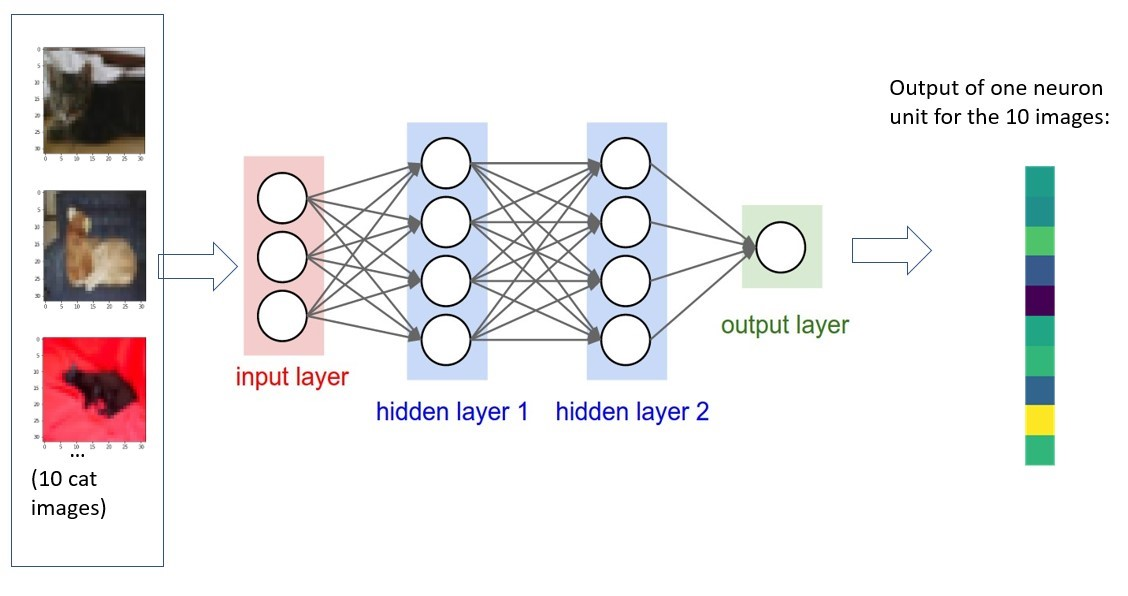
\includegraphics[width=0.7\textwidth]{figures/artificial/artificial-input-output.jpg}
            \caption{Computing output of one neuron unit in the CNNs given 10 input cat images.}
    \end{figure}
    
\begin{rmk}
At first it might seem that using different stimuli for biological and artificial neural networks will lead to an unfair comparison. However, this approach is appropriate for the following reason: The mouse visual system was trained on the flow stimuli is shown to resemble the naturalistic visual information that the mouse's vision has adapted to\footnote{Based on the paper that proposed flow stimuli \cite{visual-flow}, flow stimuli are more like what the mouse would encounter in the natural world than are sine-wave gratings but is more tractable for analysis than are natural images.}. The visual stimuli for VGG16 model came from the same data set that it is trained on (ImageNet). Thus, in both cases, the visual stimuli are similar to what the respective network was trained to recognize.
\end{rmk}
 
 \subsection{``Individual neuron" in CNN}
 In the lab experiments for biological neural networks, moving visual stimuli trigger spikes in the activation potential in the neurons in the retina. The individual neuron response is the firing rate of the neuron which is dependent on the  electrostatics processes that take place in the synapse. The biological neuron is coarsely modeled by the neuron unit in the CNNs. At the ``dendrite," the input is taken from the ``axons" of the connected neurons.\footnote{Note, however, that in our experiments, instead of taking the input from previously connected neuron unit, each neuron takes the image as the input.} The weight of each neuron models the synaptic process in biological neuron. At the ``cell body," all the inputs are multiplied with the weights and summed. We then add the bias term to the sum and apply the nonlinear activation to obtain the final output from the individual neuron unit at the ``axon." The parallel between biological and artificial neuron is shown in the figures below. 
\begin{figure}[H]
\centering
\begin{subfigure}[b]{0.5\textwidth}
        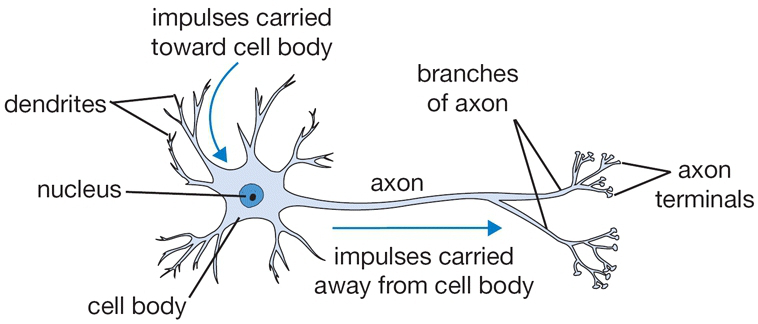
\includegraphics[width=0.9\textwidth]{figures/artificial/neuron.png}
        \caption{An individual neuron in biological neural networks. Adapted from \cite{cs231n}.}
\end{subfigure}
\hfill
\begin{subfigure}[b]{0.45\textwidth}
        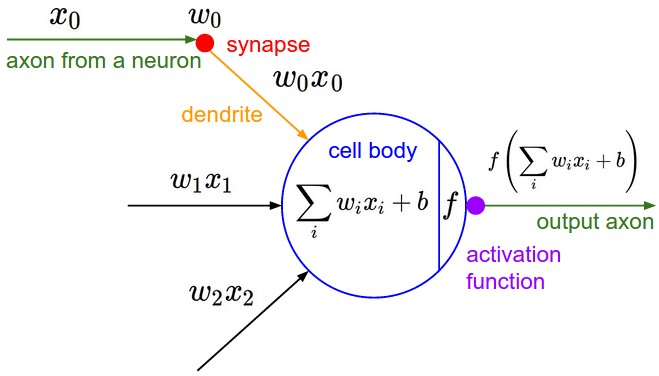
\includegraphics[width=0.9\textwidth]{figures/artificial/neuron_model.jpeg}
        \caption{An ``individual neuron" in CNNs. Adapted from \cite{cs231n}.}
\end{subfigure}
\end{figure} 

\subsection{``Receptive field" of an artificial neuron}
Each layer in the CNN has several different feature maps. Each feature map corresponds to a filter of a specific size and specific weights. The filter is essentially a matrix that, when taking inner product with the input image, give an output that highlights some specific features in the input image. To illustrate this, we can visualize the 64 feature map in the first convolutional layer of the VGG16 model, given the input image.
\begin{figure}[H]
\centering
\begin{subfigure}[b]{0.3\textwidth}
        \centering
  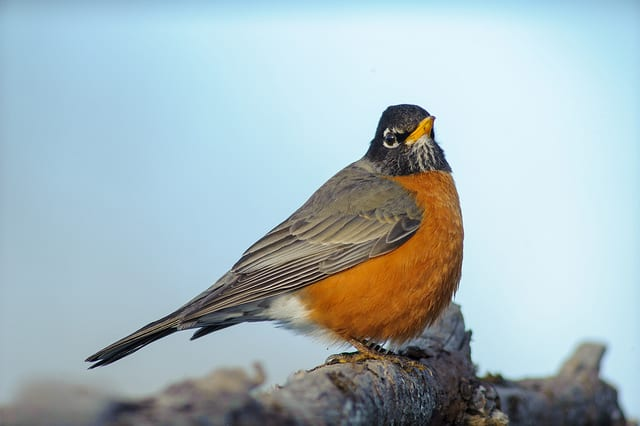
\includegraphics[width=0.6\textwidth]{figures/artificial/bird.jpg}
\caption{Input image. Adapted from \cite{feature_map}.}
\end{subfigure}
\hfill
\begin{subfigure}[b]{0.65\textwidth}
\centering
    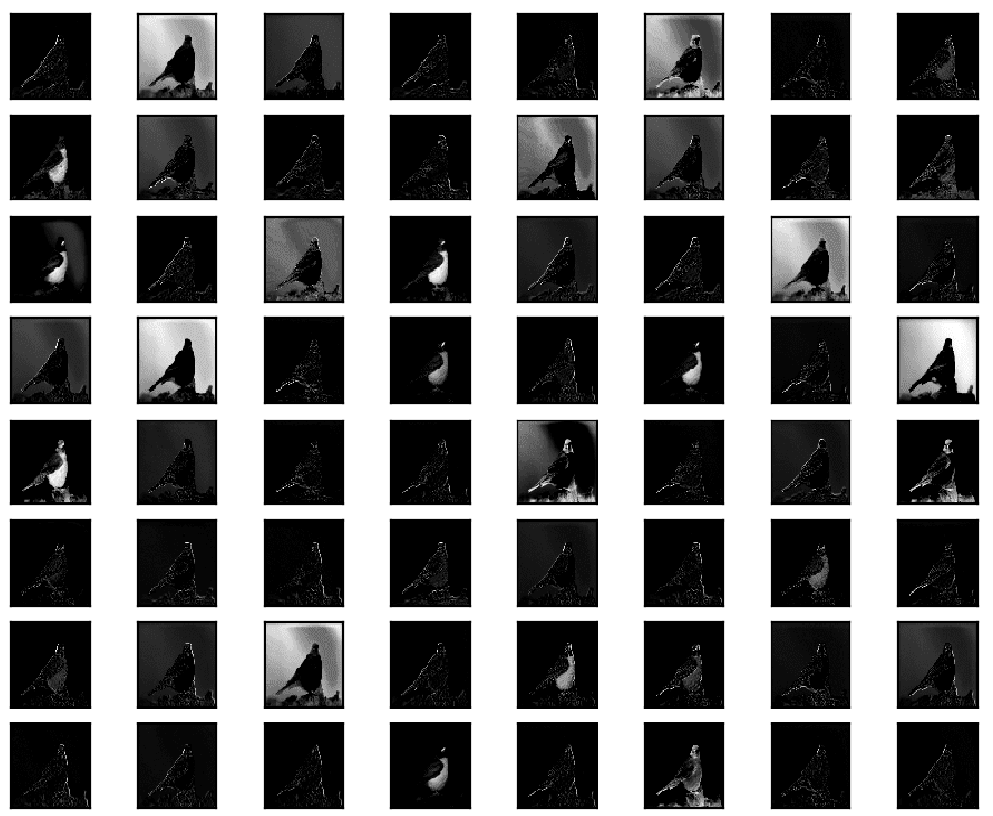
\includegraphics[width=0.45\textwidth]{figures/artificial/feature_map_vgg16.png}
    \caption{Visualizing the 64 feature maps in the first convolutional layer of the VGG16 model. Adapted from \cite{feature_map}.}
\end{subfigure}
\end{figure} 

The neurons within each feature map share the same weights and each attends to a specific subregion of the image which is referred to as their receptive field. This term originated from biological vision defined as a restricted region of visual space where a stimulus could illicit responses in a retinal ganglion cell. The size of the receptive field of a neuron is the same as the filter size corresponding to the feature map in which the neuron is located. 

 \subsection{``Neuron population response" in CNN}
Analogous to biological neural networks, we computed the neural output given the input image. Unlike biological neurons, most of the artificial neurons will have output of small values because most pre-trained weights decay to zero. In other words, the ``firing" of neurons in CNN will be sparse. We select the feature maps that contain the neurons with highest average firing rate.
% except for the specific neurons targeting at recognizing a specific features, 
% We now illustrate the dimensions of the resulting artificial neural tensor built from the first convolutional layer of VGG16. Since there were 1024 neurons in each feature map and we selected 10 feature maps, there were 10240 neurons in total. The visual stimuli consists of 10 images from each of the 10 classes, which give us 100 images. Each of the images have 1024 shifts. In the end, the size of the artificial tensor for the first convolutional layer is thus 10240-by-100-by-1024. 
\newpage
\setcounter{algocf}{1}
\begin{algorithm}[H]
\setstretch{1}
\caption{Algorithm for CNN artificial neural tensor.}\label{alg:cnn-tensor}
\DontPrintSemicolon
% Set Function Names
  \SetKwFunction{FShifts}{apply\_all\_shifts}
  \SetKwFunction{FOutput}{compute\_neuron\_output}
  \SetKwFunction{FStimuli}{show\_stimuli}
% Write Function with word ``Function''
  \SetKwProg{Fn}{Function}{:}{}
  \Fn{\FShifts{$image$, $shift\_step$}}{
        add the original image to image\_all\_shifts\;
        \For{i from 0 to \# vertical shifts}{
        shift the image vertically by shift\_step\;
        add the shifted image to image\_all\_shifts\;
            \For{j from 0 to \# horizontal shifts}{
            shift the image horizontally by shift\_step\;
            add the shifted image to image\_all\_shifts\;
            }
        }
  }
  \SetKwProg{Fn}{Function}{:}{}
  \Fn{\FOutput{$model$, $image\_all\_shifts$}}{
        \For{layer in all convolutional layers}{
        pass the image through the model\;
        take the neuron output from the specified layer after ReLU\;
        % , of shape (\# shifts, \# rows, \# columns, \# feature\_maps)\;
        % \# neurons in each feature map = \# rows * \# columns\;
        (optional) remove the neurons at the edges\;
        compute the average neuron output in each feature map\;
        select the feature maps with highest average \;
        normalize the neuron outputs in each feature map\;
        }
  }
  \SetKwProg{Fn}{Function}{:}{}
  \Fn{\FStimuli{$model$, $all\_images$}}{
        \For{image in images\_selected\_classes}{
        call \FShifts \;
        call \FOutput \;
        take average over outputs of all shifts of current image\;
        add to neuron\_output\_all\_images\;
        }
  }
\end{algorithm}

\subsection{Neural manifold for CNN}
In the plot below, each point in the data cloud represents a neuron. As shown by the disconnected clusters of neurons, the neural manifold for CNN is clearly discontinuous. When labeling the neurons according to their feature maps, we realize that these disconnected clusters are in fact organized by feature maps. This result aligns with the theoretical explanation that the neurons within the same feature map share the same filter weights. From shallow layer to deep layer, it is observed that although the clusters become more diffused, they were still form separate clusters with little overlap.

\begin{figure}[H]
\centering
\begin{subfigure}[b]{0.47\textwidth}
    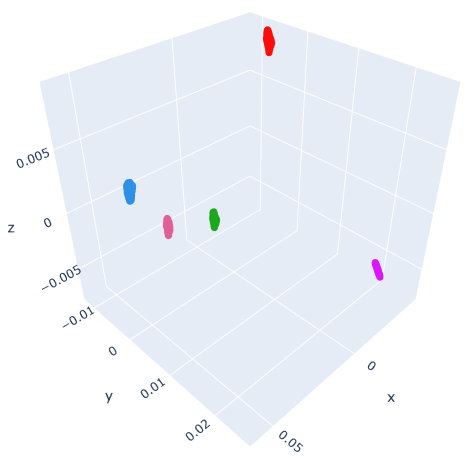
\includegraphics[width=\textwidth]{figures/embeddings/VGG16-2D-block1.png}
    \caption{VGG16 neural manifold (shallow layer).}
\end{subfigure}
\hfill
\begin{subfigure}[b]{0.45\textwidth}
    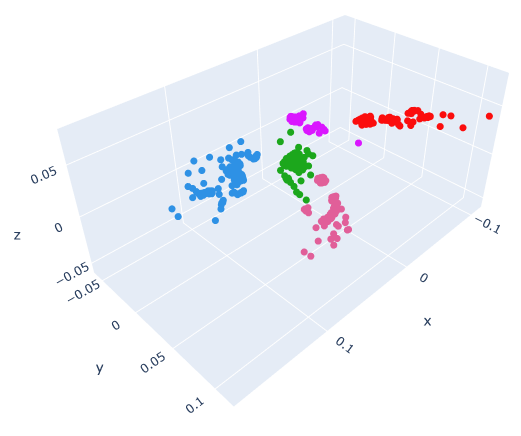
\includegraphics[width=\textwidth]{figures/embeddings/VGG16-2D-block3.png}
    \caption{VGG16 neural manifold (deep layer).}
\end{subfigure}
\end{figure}

In addition, by modifying line 24 in Algorithm \ref{alg:cnn-tensor} to appending the output for each shift instead of taking the average over all shifts, we obtain the neural manifold that preserves the spatial ordering of the neurons in the same feature map. The center and right plots below show the neurons within one cluster colored by their vertical and horizontal position. Since the neuron's coordinate on the neural manifold and the color aligns perfectly, this is good evidence that within a cluster, each neuron’s response corresponds to its spatial position given by the subregion it attends to.

\begin{figure}[H]
\centering
\begin{subfigure}[b]{0.37\textwidth}
    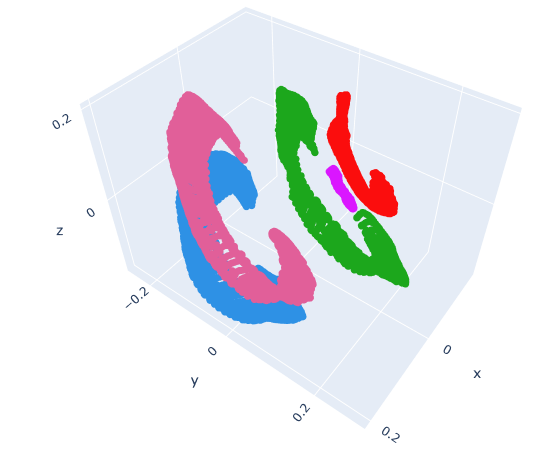
\includegraphics[width=\textwidth]{figures/embeddings/VGG16-3D-block1.png}
    % \caption{Neural manifold preserving spatial ordering.}
\end{subfigure}
\hfill
\begin{subfigure}[b]{0.3\textwidth}
    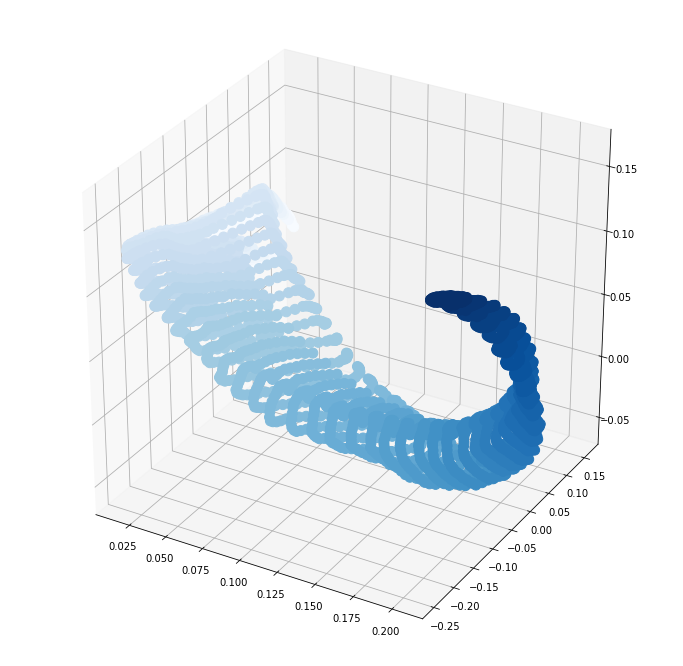
\includegraphics[width=\textwidth]{figures/embeddings/vgg16-spatial1.png}
    % \caption{Neurons colored by vertical order.}
\end{subfigure}
\hfill
\begin{subfigure}[b]{0.3\textwidth}
    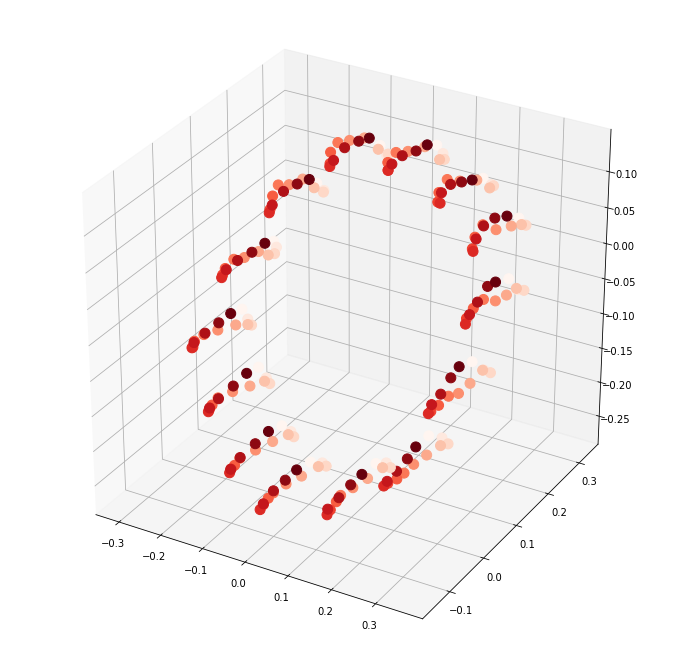
\includegraphics[width=\textwidth]{figures/embeddings/vit-spatial2.png}
    % \caption{Neurons colored by horizontal order.}
\end{subfigure}
\caption{Organization within the CNN neural manifold corresponds to neurons' spatial positions.}
\end{figure}


\section{ViT}

A recent model ViT has been shown to outperform CNN in image recognition tasks while requiring fewer computational resources \cite{vit-vs-cnn}. Transformer \cite{vaswani_attention_2017} is originally designed for sequence-to-sequence tasks primarily used in Natural Language Processing (NLP). In ViT, the given input image is divided into a sequence of 16-by-16 image patches, which allows the image recognition problem to be solved with Transformer. The distinguishing feature of the Transformer model is entirely built on the self-attention mechanisms without using sequence-aligned recurrent architecture.


\subsection{``Individual neuron" in ViTs}
The challenge in building artificial neural tensor for ViT lies in setting up a reasonable analogy to CNN. To do this, we need to scrutinize the structure of ViT. 
\begin{figure}[H]
    \centering
        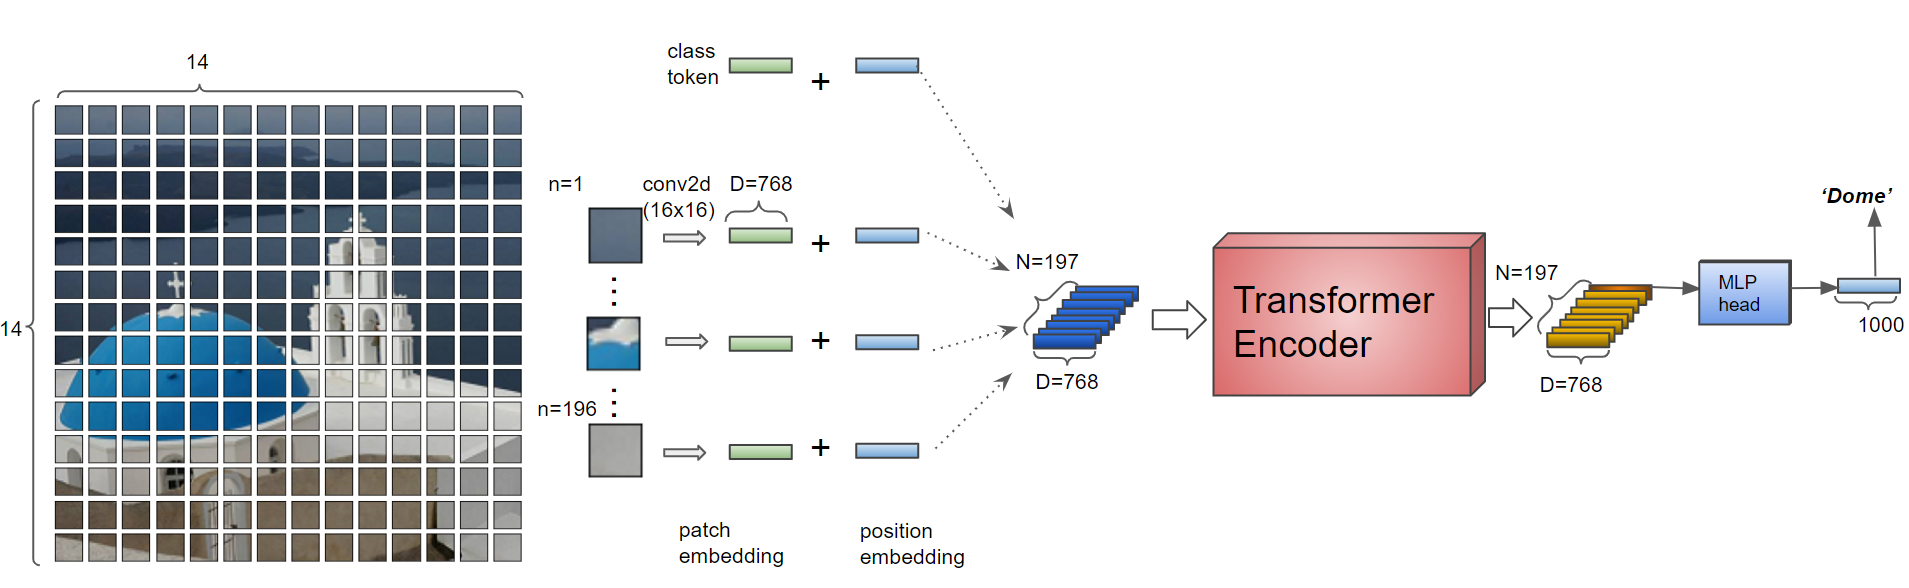
\includegraphics[width=\textwidth]{figures/artificial/vit_input.png}
        \caption{ViT input (image credit: Hiroto Honda).}
\end{figure}
    \begin{figure}[H]
    \centering
        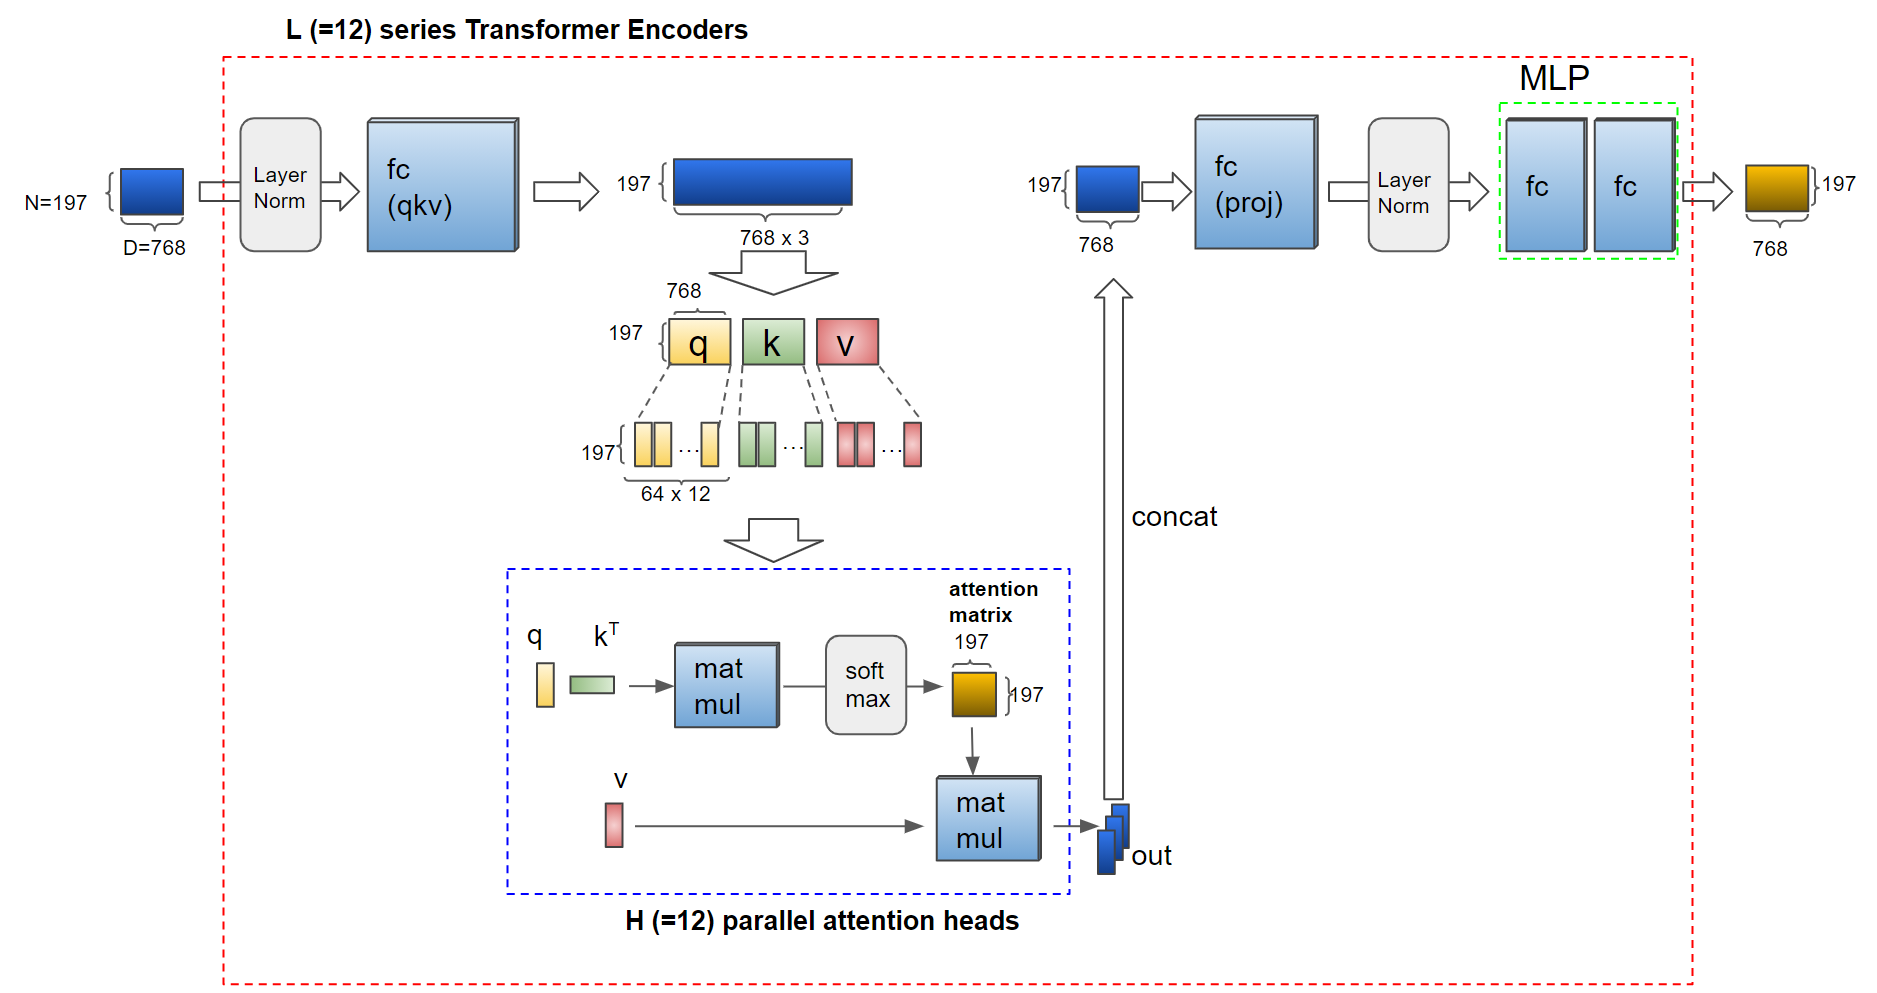
\includegraphics[width=0.8\textwidth]{figures/artificial/vit_encoder.png}
        \caption{ViT encoder (image credit: Hiroto Honda).}
\end{figure}

The following diagram compares the structures of ViT and CNN, which suggests the modification we need to make for ViT based on the previous algorithm for CNN.

\begin{figure}[H]
\centering
\begin{subfigure}[b]{0.45\textwidth}
    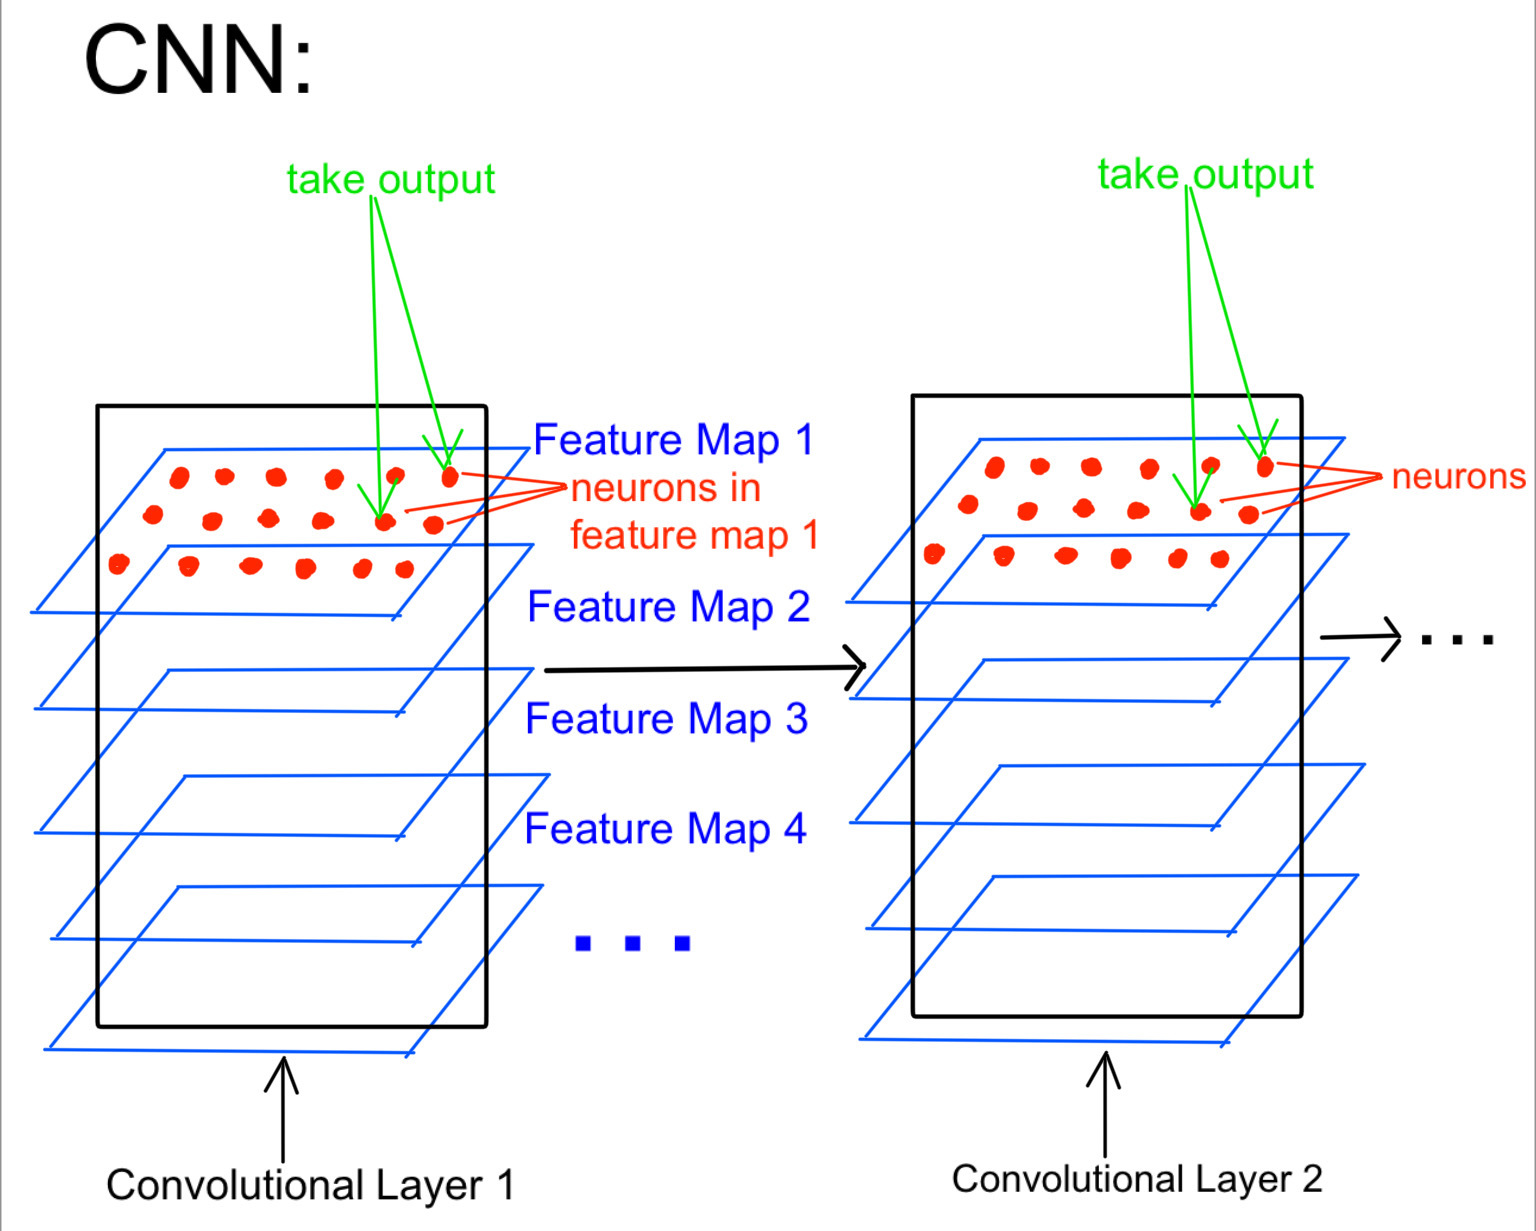
\includegraphics[width=\textwidth]{figures/artificial/cnn-tensor.jpg}
    \caption{Taking neuron output from CNN to build the corresponding neural tensor.}
\end{subfigure}
\hfill
\begin{subfigure}[b]{0.5\textwidth}
    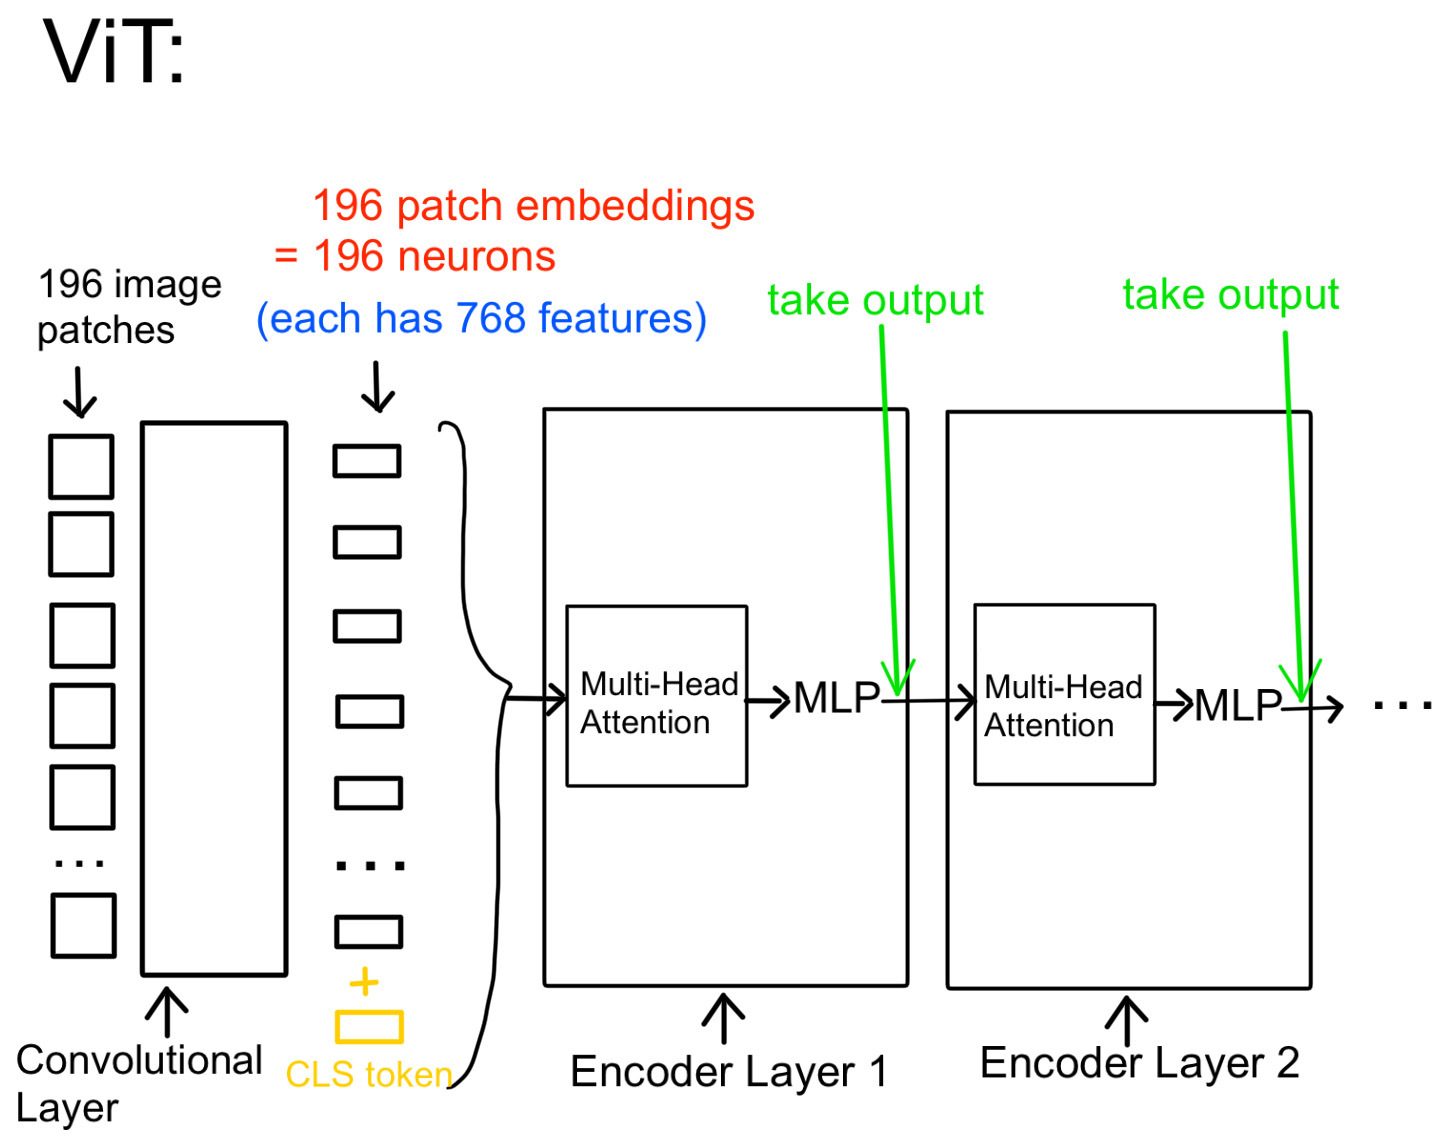
\includegraphics[width=\textwidth]{figures/artificial/vit-tensor.jpg}
    \caption{Taking neuron output from ViT to build the corresponding neural tensor.}
\end{subfigure}
\end{figure} 
Using Algorithm \ref{alg:vit-tensor}, we generate the neural manifold for ViT by taking the output from each encoder layer. The manifold structure for ViT is similar to that of CNN: the manifold is discontinuous and shows discrete clusters organized based on the features obtained from the convolutional layer before the encoder layers. 

\setcounter{algocf}{2}
\begin{algorithm}[H]
\setstretch{1}
\caption{Algorithm for ViT artificial neural tensor.}\label{alg:vit-tensor}
\DontPrintSemicolon
% Set Function Names
  \SetKwFunction{FOutput}{compute\_neuron\_output}
  \SetKwProg{Fn}{Function}{:}{}
  \Fn{\FOutput{$model$, $image\_all\_shifts$}}{
        \For{layer in all encoder layers}{
        pass the image through the model\;
        take the neuron output from the specified layer\;
        apply ReLU activation on the neuron output\;
        compute the average of neuron outputs in each feature\;
        select the feature maps with highest average \;
        normalize the neuron outputs in each feature map\;
        }
  }
\end{algorithm}

\begin{rmk}
On line 5, we need to impose ReLU\footnote{ReLU: Rectified Linear Unit \cite{relu}.} activation to make the neuron output non-negative. The non-negative constraint is desired because the tensor factors from NTF are more interpretable. The pre-trained ViT uses GELU\footnote{GELU: Gaussian Error Linear Unit \cite{gelu}.} as the activation function. This results in negative values and would prevent us from using non-negative tensor decomposition. Fortunately, the negative portion of GELU is negligible given the purpose of our investigation, which justifies this step.
\end{rmk}

An interesting observation is that from shallow layer to deep layer, the sizes of clusters mostly remain the same except for their relative positions, which is slightly different from what is observed for CNN. We provide one possible explanation for this observation. The key mechanism in ViT is self-attention while the key mechanism in CNN is convolution. A crucial difference between the two mechanisms is the receptive field size. Based on findings from \cite{raghu_vision_2021}, \cite{coatnet_2021}, convolution receptive fields are highly local and grow gradually whereas self-attention has global receptive field. As a result, ViT has more uniform representations and greater similarity between lower and deeper layers. 

\begin{figure}[H]
\centering
\begin{subfigure}[b]{0.43\textwidth}
    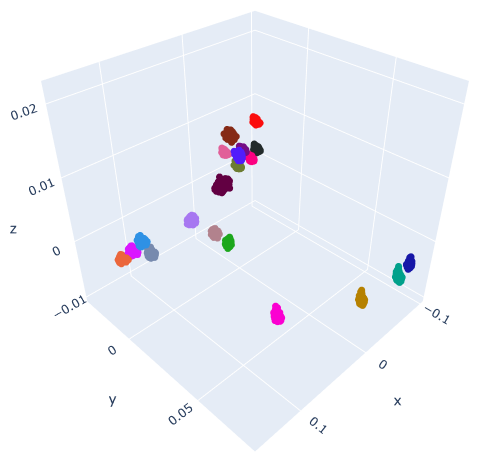
\includegraphics[width=\textwidth]{figures/embeddings/vit-2d-layer1.png}
    \caption{ViT neural manifold (shallow layer).}
\end{subfigure}
\hfill
\begin{subfigure}[b]{0.4\textwidth}
    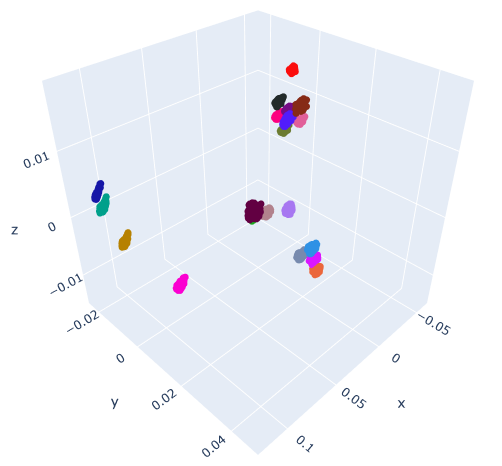
\includegraphics[width=\textwidth]{figures/embeddings/vit-2d-layer12.png}
    \caption{ViT neural manifold (deep layer).}
\end{subfigure}
\end{figure}

We also visualize the neural manifold for ViT that preserves the spatial information, which shows that similar to CNN, neuron responses in ViT also have similar spatial organization within the neural manifold. This similarity is likely because ViT encoder layer takes the features from the convolutional layer as its input.
\begin{figure}[H]
\centering
\begin{subfigure}[b]{0.37\textwidth}
    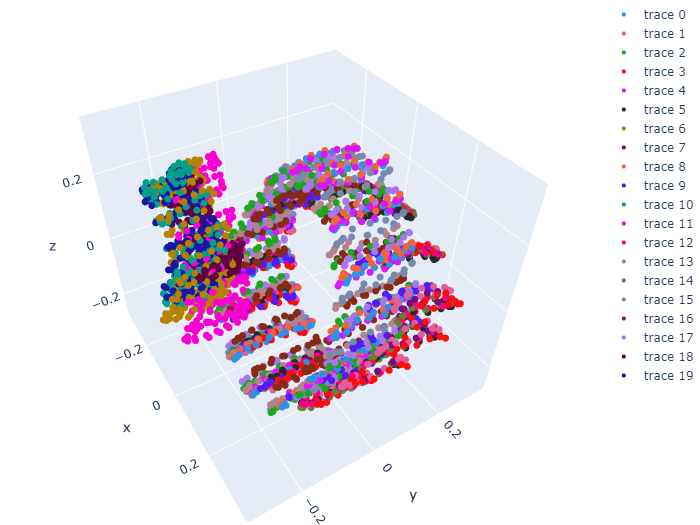
\includegraphics[width=\textwidth]{figures/embeddings/vit-3d-layer1.png}
    % \caption{Neural manifold preserving spatial ordering.}
\end{subfigure}
\hfill
\begin{subfigure}[b]{0.3\textwidth}
    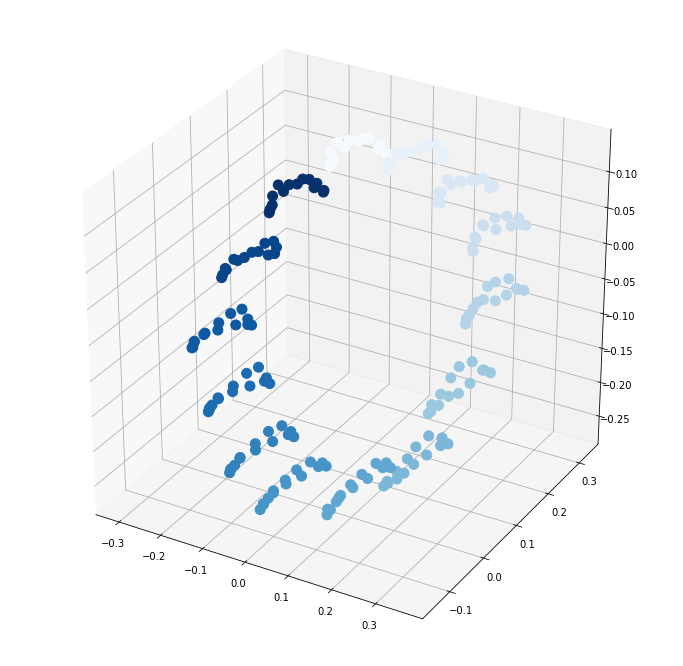
\includegraphics[width=\textwidth]{figures/embeddings/vit-spatial1.png}
    % \caption{Neurons colored by vertical order.}
\end{subfigure}
\hfill
\begin{subfigure}[b]{0.3\textwidth}
    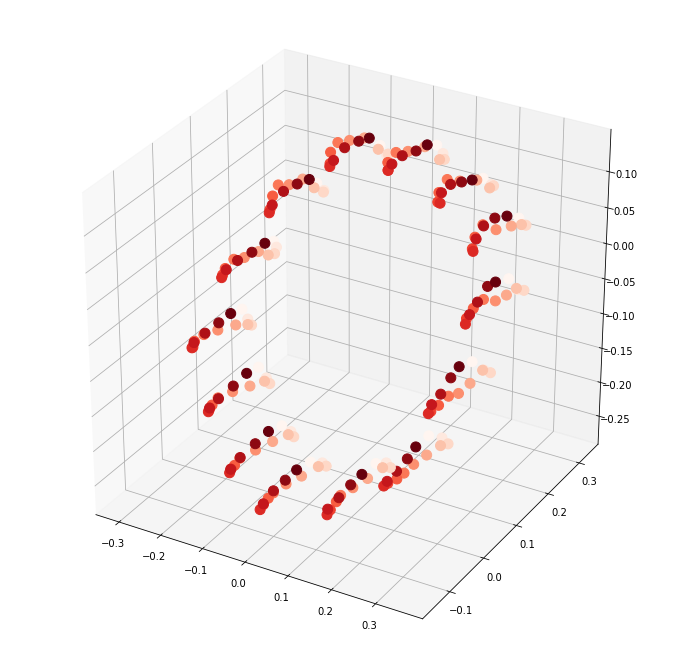
\includegraphics[width=\textwidth]{figures/embeddings/vit-spatial2.png}
    % \caption{Neurons colored by horizontal order.}
\end{subfigure}
\caption{Organization within the ViT neural manifold corresponds to neurons' spatial positions.}
\end{figure}

\subsection{Quantifying the continuity of the manifold}

Following the method proposed in \cite{dyballa_manifold_2021}, we further compute the MFR as we have done for biological neural networks. Since it is clear from the visualization that the neural manifolds CNN and ViT are similarly discontinuous, it suffices to compute the MFR for one of them. We compare the respective neural manifolds and their respective MFR for CNN, retina, and V1:

\begin{figure}[H]
\centering
\begin{subfigure}[b]{0.3\textwidth}
        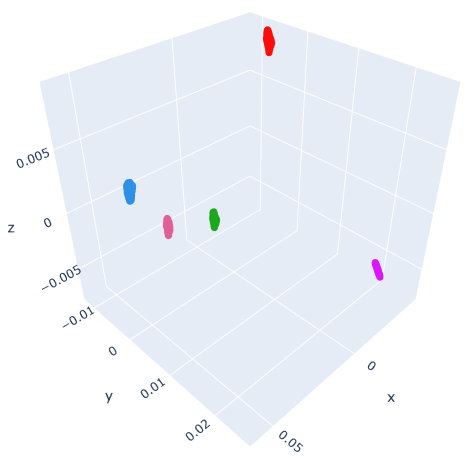
\includegraphics[width=\textwidth]{figures/embeddings/VGG16-2D-block1.png}
        \caption{$\phi_G = 0.27$ for CNN.}
\end{subfigure}
\hfill
\begin{subfigure}[b]{0.3\textwidth}
        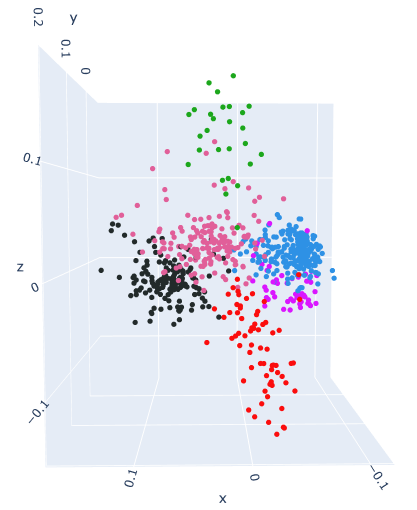
\includegraphics[width=\textwidth]{figures/biological/retina-manifold.png}
        \caption{$\phi_G = 0.56$ for retina.}
\end{subfigure}
\hfill
\begin{subfigure}[b]{0.3\textwidth}
        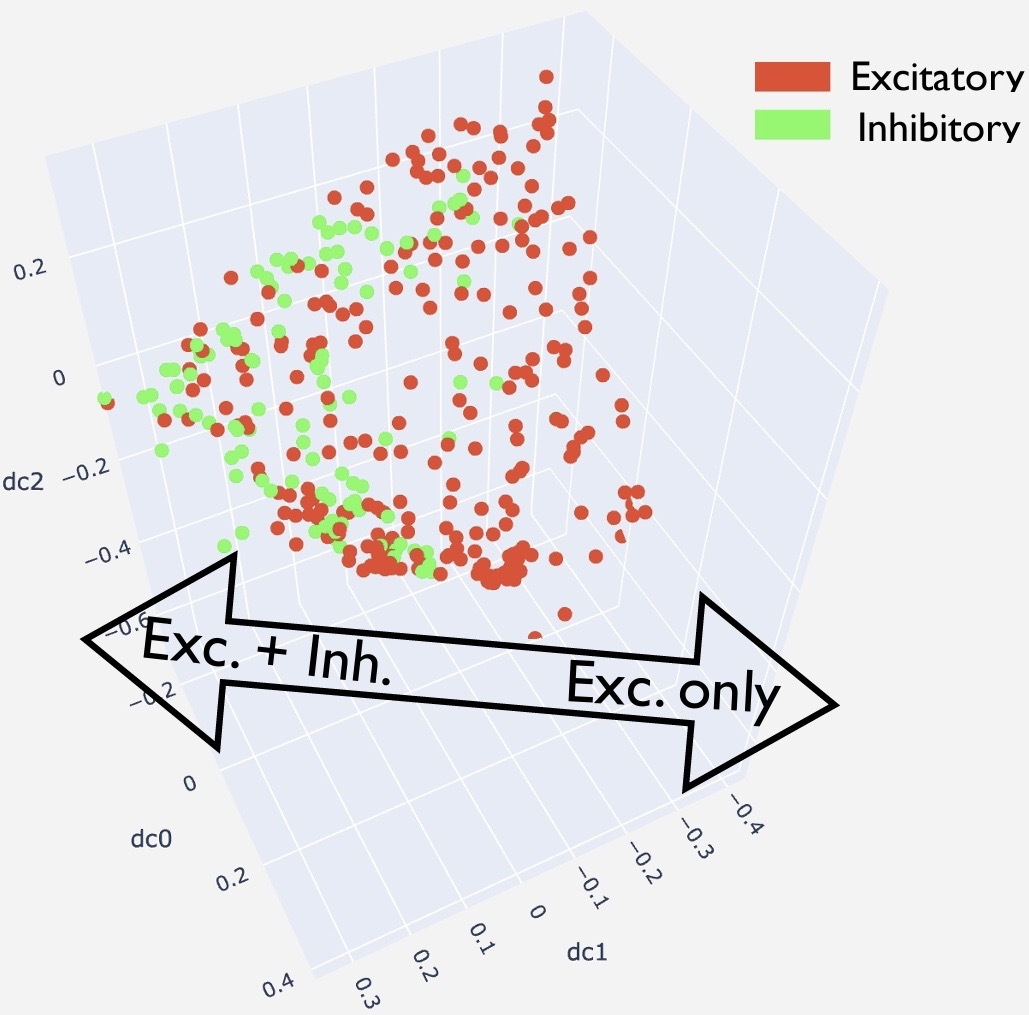
\includegraphics[width=\textwidth]{figures/biological/v1-manifold.jpg}
        \caption{$\phi_G = 0.91$ for V1.}
\end{subfigure}
\end{figure} 
% \begin{figure}[H]
% \centering
%     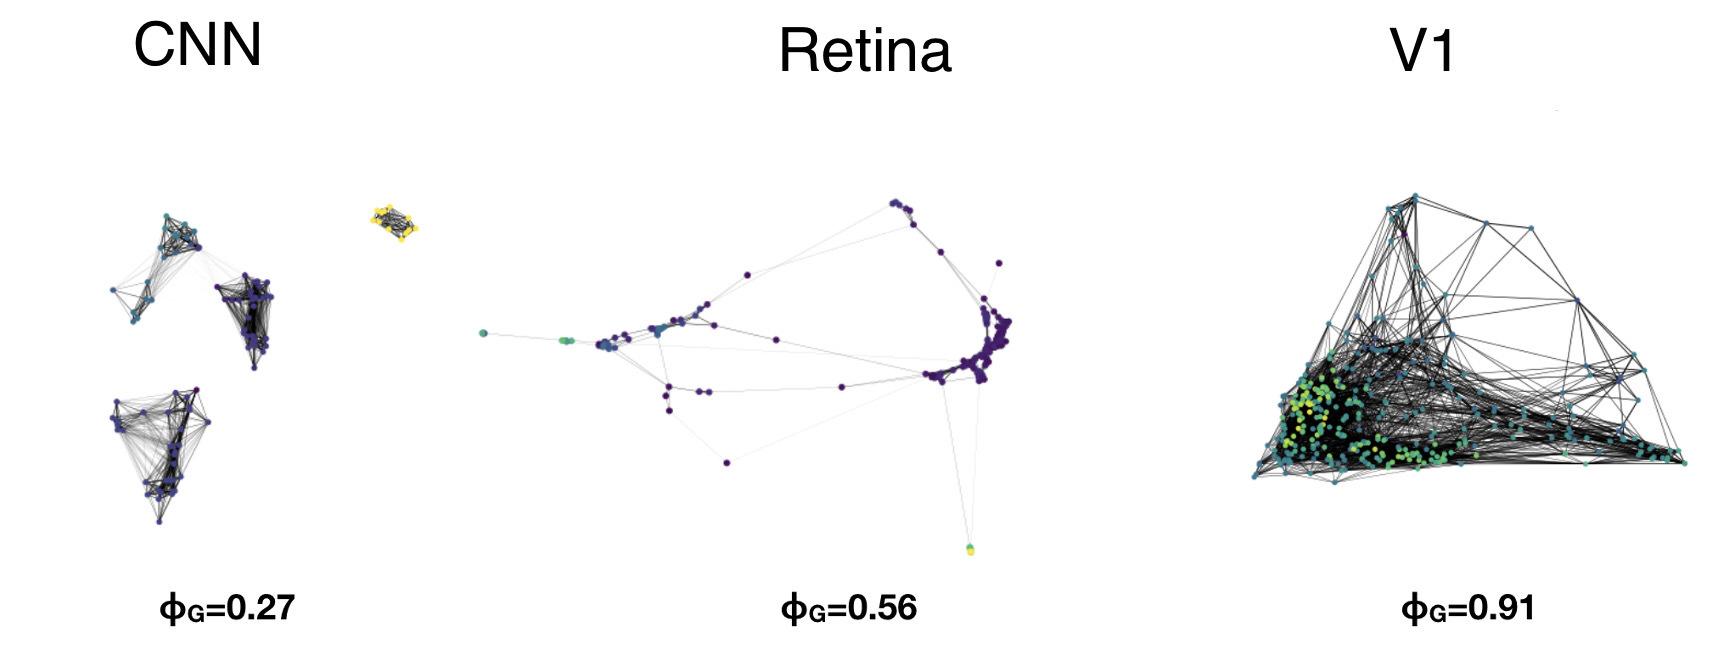
\includegraphics[width=0.75\textwidth]{figures/embeddings/mean-flow-ratio-results.jpg}
% \caption{Comparing the mean flow ratio of CNN with that of the biological neural networks in retina and V1.}
% \end{figure}
The quantitative comparison aligns with our qualitative comparison: from the visualization, we have observed that V1 has a much more continuous manifold than CNN and the retina; similarly, the MFR of V1 is notably higher than CNN and the retina. MFR additionally reveals (which is not entirely obvious from the visualizations) that there seems to be a considerable gap between between CNN and retina as well.

\section{Adding recurrence}
Since neither the convolution in CNN nor the attention mechanism in ViT yields continuous neural manifold like V1, this leads us to investigate other computational mechanisms that could result in a more continuous neural manifold. Based on our literature review in \ref{neuro-recurrent}, we hypothesize that recurrent models might be promising. For this reason, we apply the same method to investigate computer vision models with recurrent structures. One challenge is that recurrent neural networks (RNNs) themselves are not commonly used for image recognition tasks. Fortunately, there are computer vision models that combine convolution and recurrent units. For this reason, we choose two representative models: first, convolutional RNN (CRNN) \cite{convrnn_shi_end--end_2015} that adds recurrent layers after the convolutional layers and second, $\gamma$-net \cite{serre-recurrence} that adds recurrent connections directly on the convolutional layers. Algorithm \ref{alg:cnn-tensor} for CNN applies in this case as well. We include here our preliminary findings for neural manifold obtained from CRNN \cite{convrnn_shi_end--end_2015}.  
\begin{figure}[H]
\centering
    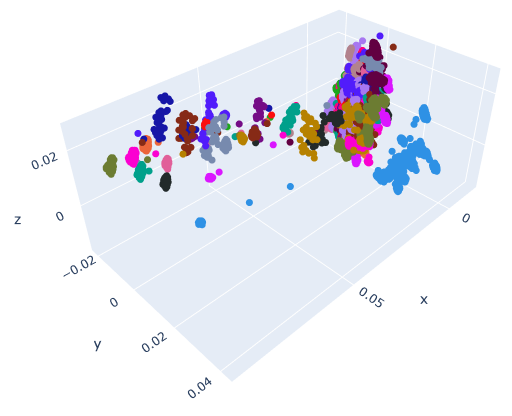
\includegraphics[width=0.5\textwidth]{figures/embeddings/crnn-2d-layer1.png}
\caption{Neural manifold for CRNN (shallow layer).}
\end{figure}
As observed from the figure above, the clusters become less separated and  ignificantly overlap with each other, which is in contrast to the neural manifolds for CNN and ViT . This suggests that by adding the recurrently layers and jointly training the unified network we can obtain a more continuous manifold. A possible reason for this observation is that due to the structure of this model, the convolutional layers are affected by the recurrent units in the RNN layers in that the RNN layers can back-propagate error differentials to its inputs from the convolutional layers. 

Another intriguing result is that when visualizing the neural factors (obtained by applying NTF on respective neural tensors), the neural factors for CRNN seem to have very distinct properties from those for CNN and ViT. The neural factors visualize the independent neural firing patterns that can approximately summarize all the neural firing patterns in the original neural tensor. In the following figure, we see that the for CNN and ViT there is mostly just one bright region in each factor, suggesting that the neurons mostly respond to a single targeted feature/region in the input image. This likely implies the neurons have strong stimuli preferences and they participate in isolated neural circuits (thus yielding a continuous manifold). However, neural factors for CRNN indicate some sequential patterns with many bright regions in each factor, suggesting that the neurons might respond to multiple stimuli. This implies that the underlying neural circuit is more interconnected, which is why we have observed a more continuous manifold.
\begin{figure}[H]
\centering
\begin{subfigure}[b]{0.4\textwidth}
        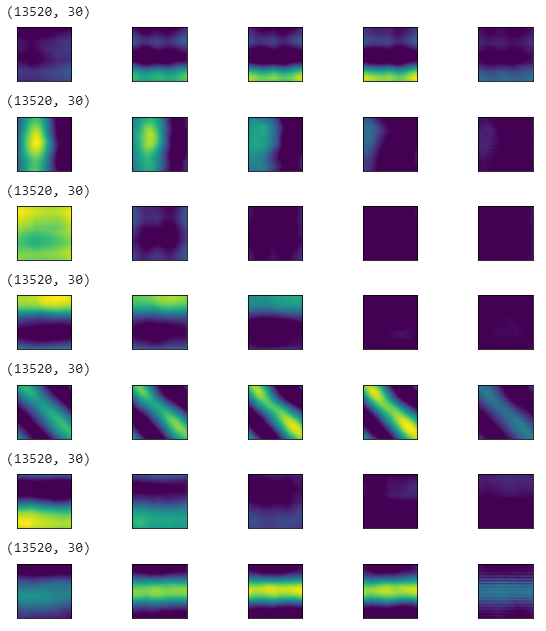
\includegraphics[width=0.85\textwidth]{figures/artificial/cnn-factor.PNG}
        \caption{Neural factors for CNN.}
\end{subfigure}
\hfill
\begin{subfigure}[b]{0.57\textwidth}
        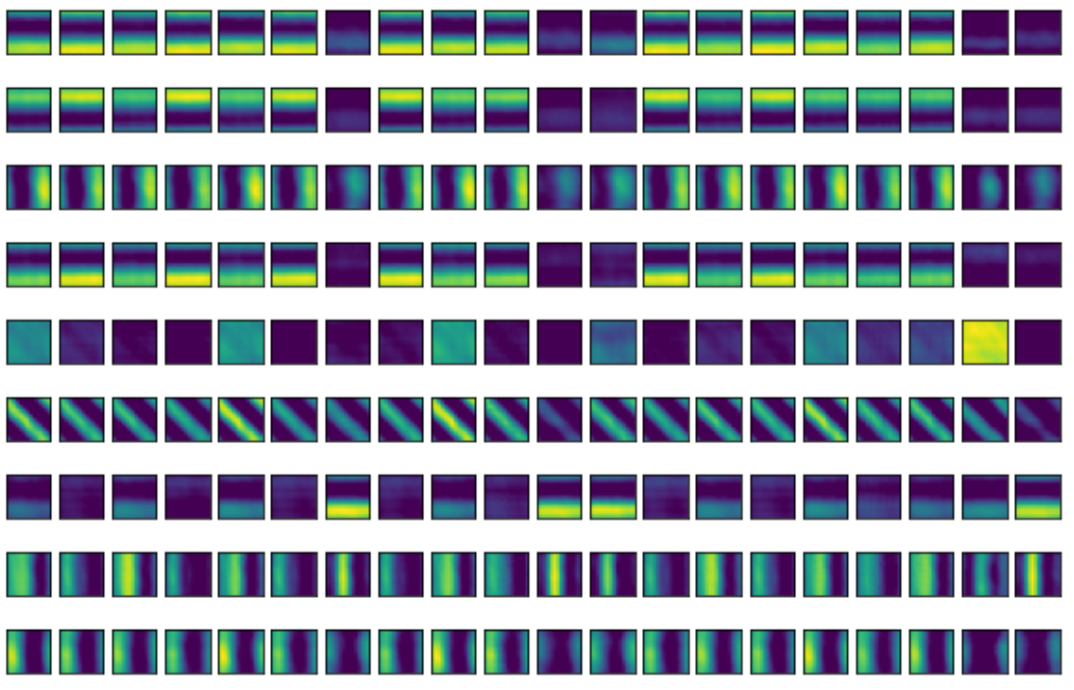
\includegraphics[width=\textwidth]{figures/artificial/vit-factor.PNG}
        \caption{Neural factors for ViT.}
\end{subfigure}
\end{figure} 
\begin{figure}[H]
\centering
    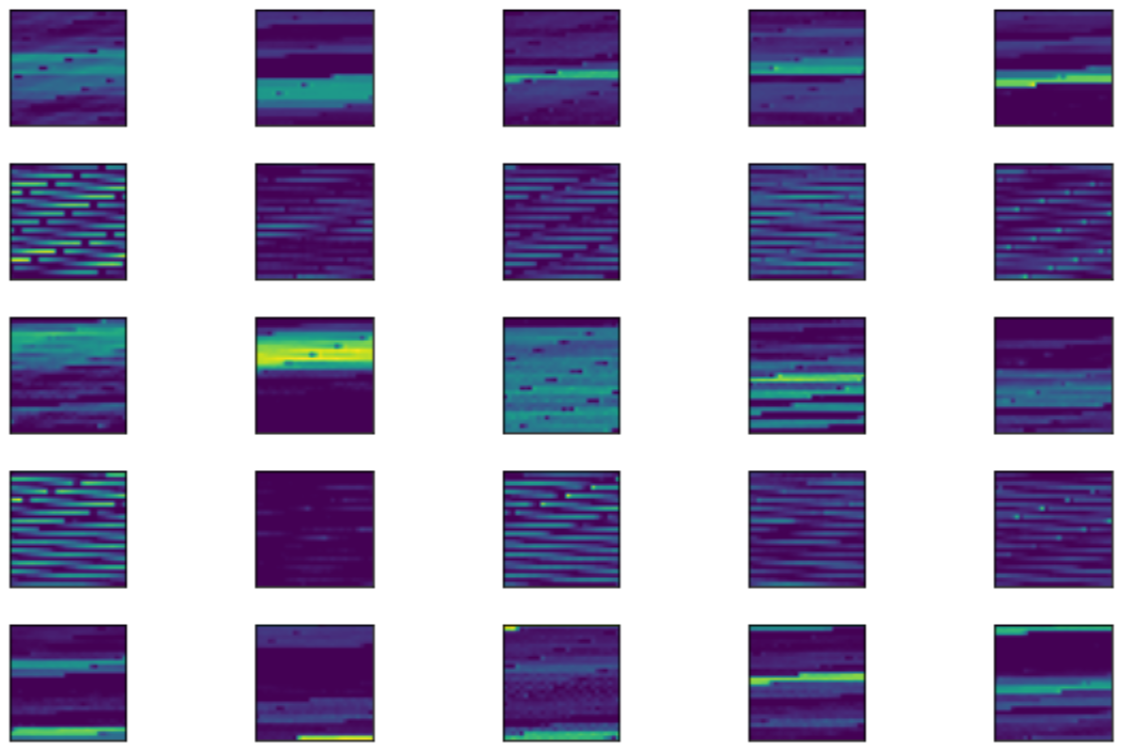
\includegraphics[width=0.45\textwidth]{figures/artificial/crnn-factor.png}
    \caption{Neural factors for CRNN are distinct from CNN and ViT.}
\end{figure}
